	  Теперь докажем частный случай известно <<неприятной леммы>>, которая понадобится нам в дальнейшем. 

	  \begin{lemma}[Ugly lemma]
	  	Пусть $G$~--- конечная группа, $A \in G\text{-}\Mod$ и выполнены следующие условия 

	  	\begin{enumerate}
	  		\item Для любой подгруппы $H \le G$  тривиальны первые когомологии $H^{1}(H, A) = 0$.

	  		\item Если $H \le K$~--- нормальная подгруппа в подгруппе $K \le G$ и $|K/H| = p$ (где $p$~--- простое), то 
	  		\[
	  			|H^2(K/H, A^H)| \ \mid \ p .
	  		\]
	  	\end{enumerate}

	  	Тогда $|H^2(G, A)| \ \mid \ |G|$. 
	  \end{lemma}
	  \begin{proof}
	  	\noindent\bf{Шаг 1.} Предположим, что $G$~--- это $p$-группа. Будем вести индукцию по $|G|$.

	  	\noindent\bf{База.} Случай $|G| = 1$ очевиден. 

	  	\noindent\bf{Переход.} В $G$ существует нормальная подгруппа $H$ индекса $p$. По индукционному предположению $|H| \divby |H^2(H, A)|$. Запишем точную последовательность для ограничения и инфляции: 
	  	\[
	  		0 \to H^2(G/H, A^H) \xrightarrow{\inf} H^2(G, A) \xrightarrow{\res} H^2(H, A) 
	  	\]

	  	Соответственно, из неё мы заключаем, что 
	  	\[
	  		\begin{cases} p  = |G/H| \divby |H^2(G/H, A^H)|  \text{ (по условию теоремы)}\\ |H| \divby |H^2(H, A) |\end{cases} \implies |G| \divby |H^2(G, A)|. 
	  	\]

	  	\noindent\bf{Шаг 2.} Теперь рассмотрим общий случай. Как мы помним из следствия~\ref{Sylow_subgroups_mono}, отображение 
	  	\[
	  		\widehat{H}^q(G, A) \xrightarrow{\bigoplus \res_{G/S_p}} \bigoplus_{p} \widehat{H}^{q}(S_p, A)
	  	\]
	  	является мономорфизмом. Отсюда мы заключаем, что 
	  	\[
	  		 \left\lvert \bigoplus_{p} \widehat{H}^{2}(S_p, A) \right\rvert \divby |H^2(G, A)|.
	  	\]
	  	С другой стороны, по первому пункту мы знаем, что $|S_p| \divby |\widehat{H}^{2}(S_p, A)|  $, откуда 
	  	\[
	  		|G| = \prod_{p} |S_p|  \divby \prod_{p} |\widehat{H}^{2}(S_p, A) | \divby  |H^2(G, A)|,
	  	\]
	  	чего мы собственно и хотели. 

	  \end{proof}

	  Теперь применим эту замечательную "неприятную" лемму в нашем контексте. Пусть $G = \Gal(L/K)$, $A = L^*$. 

	  \begin{enumerate}
	  	\item По соответствию Галуа, любой подгруппе $H \le G$ соответствует $E/K, \ E \subset L$, причём $\Gal(L/E) = H$. 

	  	\begin{center}
	  		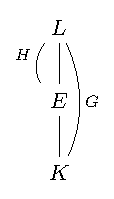
\includegraphics{lectures/6/pictures/cd_27.pdf}
	  	\end{center}

	  	По теореме Гильберта-90 $H^1(H, L^*) = 0$. Это гарантирует нам выполнение первого условия неприятной леммы. 

	  	\item Теперь, второму условию в неприятной лемме соответствует такая башня полей: 
	  	\begin{center}
	  		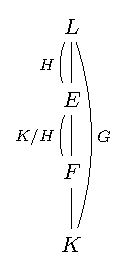
\includegraphics{lectures/6/pictures/cd_28.pdf}
	  	\end{center}

	  	Соответственно, по определению группы Галуа: $A^H = (L^*)^H = E^*$ и тогда соответственно 
	  	\[
	  		H^2(K/H, A^H) \cong H^2(K/H, E^*) \cong H^2(\Gal(E/F), E^*).
	  	\]
	  	Так как группа Галуа $\Gal(E/F)$ циклическая, по доказанному ранее (см.~\ref{max_nerazvetv_ext})
	  	\[
			p = |\Gal(E/F)|	  \divby |H^2(K/H, A^H)|.		
	  	\]
	  \end{enumerate}

	  Тогда по неприятной лемме мы получаем, что 
	  \[
	  	|G| \divby |H^2(G, A)|.
	  \]

	Итого, мы доказали такую теорему 

	\begin{theorem} 
		Пусть $L/K$~--- конечное расширение локального поля $K$ с группой Галуа $G = \Gal(L/K)$. Тогда 
		\[
			|G| = [L : K] \divby |H^2(G, L^*)|.  		
	  	\]  	
  	\end{theorem}	  

  	\subsubsection{Группа $H^2(G, L^*)$ в общем случае для локального поля}

  	Рассмотрим короткую точную последовательность  $G$-модулей с тривиальным действием
  	\[
  		0 \to \Z \hookrightarrow \Q \twoheadrightarrow \Q/\Z \to 0
  	\]

  	Она индуцирует длинную точную последовательность когомологий 
  	\[
  		\ldots \widehat{H}^{q - 1}(G, \Q/\Z) \to \widehat{H}^q(G, \Z) \to \widehat{H}^q(G, \Q) \to \widehat{H}^{q}(G, \Q/\Z) \to \widehat{H}^{q + 1}(G, \Z) \to \ldots 
  	\]

  	Заметим, что умножение на $|G|$ индуцирует изоморфизм $\Q \xrightarrow{\sim} \Q$, а он индуцирует отображение 
  	\[
  		\widehat{H}^{q}(G, \Q) \xrightarrow[\cdot |G|]{\sim} \widehat{H}^{q}(G, \Q)
  	\]
  	. С другой стороны, мы знаем, что $|G| \cdot \widehat{H}^q(G, \Q) = 0$. Отсюда мы заключаем, что 
  	\[
  		\widehat{H}^q(G, \Q) = 0.
  	\]

  	Тогда из длинной точной последовательности пары выше мы видим, что 
  	\[
  		\widehat{H}^1(G, \Q/\Z) \cong \widehat{H}^2(G, \Z).
  	\]
  	Посмотрим внимательнее на группу $H^{1}(G, \Q/\Z) \cong \Z^{1}(G, \Q/\Z)/B^1(G, \Q/\Z)$. Как мы помним, кограницы~--- это функции $\varphi\colon G \to \Q/\Z$, для которых существует $a \in \Q/\Z$ такой, что $\varphi(g) = ga - a$. Но, так как действие тривиально, $\varphi(g) = ga - a = a - a = 0$, откуда $B^1(G, \Q/\Z) = 0$. Кроме того, $\Z^{1}(G, \Q/\Z)$~--- это скрученные гомоморфизмы $\varphi\colon G \to \Q/\Z$, т.е. отображения вида 
  	\[
  		\varphi(g_1 g_2) = g_1 \varphi(g_2) + \varphi(g_1) = \varphi(g_2) + \varphi(g_1),
  	\]
  	так как действие тривиально. Соответственно, $Z^1(G, \Q/\Z) = \Hom_{\Grp}(G, \Q/\Z)$. Значит, 
  	\[
  		H^1(G, \Q/\Z) \cong \Hom(G, \Q/\Z). 
  	\]
  	Соответственно, мы получили, что 
  	\[
  		H^2(G, \Z) \cong \Hom(G, \Q/\Z).
  	\]

  	\begin{example}
  		Пусть $G = \langle \sigma \rangle$~--- циклическая группа. Пусть $|G| = m$. Рассмотрим отображение 
  		\[
  			\sigma \mapsto \frac{1}{m}
  		\]
  		индуцирует изоморфизм  $\Hom(G, \Q/\Z) \cong \frac{1}{m}\Z/\Z$. 
  	\end{example}

  	Пусть теперь $L/K$~--- неравзетвлённое расширение локального поля $K$. Тогда 
  	\[
  		\Gal(L/K) \cong \Gal(\ell/\Bbbk)
  	\]
  	и, если $|\Bbbk| = q$, то группа $\Gal(\ell/\Bbbk$ порождена автоморфизмом Фробениуса 
  	\[
  		\Fr_q\colon \ell \to \ell, \ \Fr_q(x) = x^q.
  	\]

  	При изоморфизме этот автоморфизм переходит в некоторый элемент $F \in \Gal(L/K)$, причем такой, что 
  	\[
  		F(x) \equiv x^q \pmod{\fm_{L}} \text{ для } x \in \cO_{L}.
  	\]

  	Допуская волность речи, этот элемент мы также будем называть автоморфизмом Фробениуса. 

  	Теперь пусть $L/K$~--- расширение Галуа локального поля $K$ степени $[L : K] = |G| = n$. Рассмотрим $K_m/K$~--- неравзетвлённое расширение поля $K$ степени $m$. Рассмотрим композит расширений 
  	\begin{center}
  		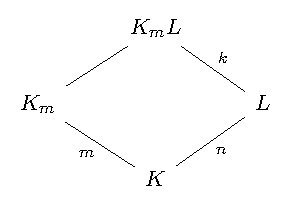
\includegraphics{lectures/6/pictures/cd_29.pdf}
  	\end{center}

  	Тогда у нас есть вот такая коммутативная диаграмма: 

  	\begin{center}
  		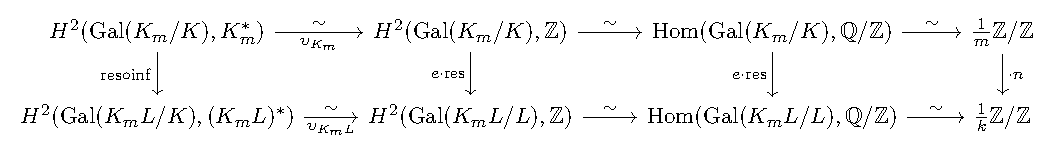
\includegraphics{lectures/6/pictures/cd_30.pdf}
  	\end{center}

  	Поясним, что на ней вообще происходит. 

  	\begin{itemize}
  		\item Первое вертикальное отображение происходит из точной последовательности для ограничения и инфляции. Если конкретнее, то у нас есть такая башня: 

  		\begin{center}
  			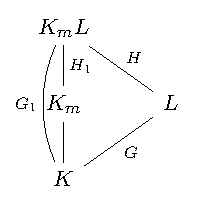
\includegraphics{lectures/6/pictures/cd_31.pdf}
  		\end{center}

  		И из неё мы получаем отображение 

  		\[
  			  H^2(G_1/H_1, K_m^*) \xrightarrow{\inf} H^2(G_1, (K_m L)^*) \xrightarrow{\mathrm{res}} H^2(H_2, (K_m L)^*)
  		\]

  		И в качестве стрелки мы берём сквозное отображение.

  		\item Вторую вертикальную стрелку мы на самом деле уже видели. А именно, у нас есть кроткая точная последовательность  
  		\[
  			1 \to U_{K_m} \to K_m^* \xrightarrow{\v_{K_m}} \to \Z \to 0,
  		\]
  		а так как (как мы видели в вычислении для неравзетвлённого расширения) $\widehat{H}^{1}(\Gal(K_m/K), U_{K_m}) = 0$, мы получаем изоморфизм $\widehat{H}^2(\Gal(K_m/K), K_m^*) \cong \widehat{H}^2(\Gal(K_m/K), \Z)$.

  		Аналогично и для нижнего куска диаграммы, так как мы доказывали, что если расширение $K_m/K$ неразветвлено и является подрасширением в $L$, то $K_m L / L$ неравзетвлено. 

  		\item Третья вертикальная стрелка получается из обсуждённого только что изоморфизма 
  		\[
  			H^2(G, \Z) \cong \Hom(G, \Q/\Z).
  		\]

  		\item Четвёртая вертикальная стрелка также получается из рассуждения выше про $\Hom(G, \Q/\Z)$ для циклической группы (а тут она именно такова, так как расширение неразветвлено). 
  	\end{itemize}

  	Поясним теперь, почему эта диаграмма коммутативная. 

   Пусть $e = e(L/K)$. Коммутативность левого квадрата следует из того, что 
  	\[
  		\forall x \in K_m^* \quad e \cdot \v_{K_m}(x) = \v_{K_m L}(x),
  	\]
  	так как $e(K_m L/K_m) = e(L/K)$. Соответственно, в частности для 2 коциклов выполнено 
  	\[
  		e \v_{K_m}(f(\sigma_1, \sigma_2)) = \v_{K_m L}(f(\sigma_1, \sigma_2)). 
  	\]

  	Коммутативность второго квадрата следует из согласованности ограничения с длинной точной последовательностью. Коммутативность третьего квадрата следует из того, что 
  	\[
  		n \varphi(F_K) = e \cdot \varphi(F_L),
  	\]
  	где $F_K$~--- автоморфизм Фробениуса. Это в свою очередь равносильно тому, что $f(L/K) \cdot \varphi(F_k) = \varphi(F_L)$ (так как $n = ef$), а это выполнено так как $F_L = F_K^{f}$, где.

  	Возьмём теперь $m = n$. В этом случае правое отображение будет нулевым, откуда крайнее левое~--- тоже. В то же время,  в силу теоремы Гильберта-90 последовательность 2-х когомологий для ограничения и инфляции точна
  	\[
  			0 \to H^2(\Gal(L/K), L^*) \xrightarrow{\inf_2} H^2(\Gal(K_m L/K), (K_m L)^*) \xrightarrow{\mathrm{res}} H^2(\Gal(K_m L/L), (K_m L)^*)
	\]

	(и заметим, что тут имеется в виду другое отображение инфляции между другими группами!). 

  	 Соответственно, мы получаем вот такую коммутативную диаграмму: 

  	 \begin{center}
  	 	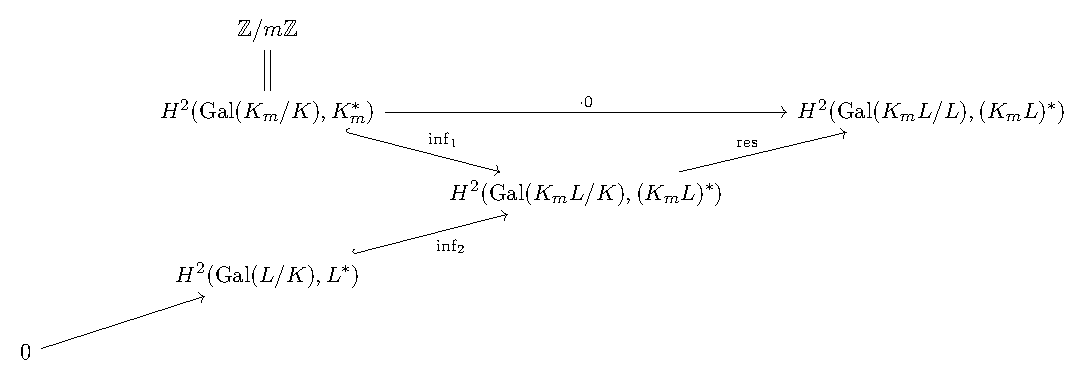
\includegraphics{lectures/6/pictures/cd_32.pdf}
  	 \end{center}

  	 Из этой диаграммы мы получаем, что  $\Z/m\Z \hookrightarrow H^2(\Gal(L/K), L^*)$.. С другой стороны, из неприятной леммы мы знаем, что $m = n \divby |H^2(\Gal(L/K), L^*)| $, откуда 
  	 \[
  	 	H^2(G, L^*) \cong \Z/m\Z.
  	 \]
  	 Итак, мы наконец доказали вот такую теорему: 

  	 \begin{theorem} 
  	 	Пусть $L/K$~--- конечное расширение Галуа локального поля $K$ степени $n$ с группой Галуа $\Gal(L/K) = G$. Тогда 
  	 	\[
  	 		H^2(G, L^*) = \Z/n\Z.
  	 	\]
  	 \end{theorem}

    \subsection{Группа Брауэра}

    \textcolor{red}{Этот параграф будет добавлен после девятой и десятой лекций. }
    
  	 












	  



	  












	  



	  
